Model in hand, we are finally ready to start tuning its hyperparameters on a dataset.
Where to start?
First, we processed the FER2013 dataset, with mean image substraction, and a 1200 images validation set.
Then, we define the classification accuracy on the validation set as
the performance measure to be used to compare the performance of the different parameters on the validation set.

\begin{itemize}[topsep=-10pt]
\item \textbf{Select a reasonable network architecture}:\\
  After some hand-tuning of the hidden layer size, we decided to start with a single hidden layer of 256 hidden units.
  It seemed a reasonable tradeoff between complexity and training efficiency, and less likely to overfit.
  We set our model's momentum to 0.9 and its learning rate to a relatively small 1e-6
  since the magnitude of the gradient will be larger due to momentum.
  We trained for 15 epochs with batch size of a 100.
  We added the following stopping criterion: stop if the error in the validation set does not decrease for three consecutive cycles,
  and stop if the loss diverges to ``nan''.
  This will help increase our training efficiency.

\item \textbf{Optimize the learning rate}:\\
  Our experience hand-tuning the network as mentioned gave us a better idea of the range of learning rates we should test.
  We decided to initiate a grid search (of one parameter) for the learning rate in the range (1e-7, 1e-3).
  using the parameters found through hand-tuning in the previous section.
  Please find a below a graph showing the best validation accuracy for each learning rate tested in the range.
  \begin{figure}[!ht]
      \centering
      {{\includegraphics[scale = 0.50]{../src/optimizers/outputs/grid_search/learning_rate.png}}}
  \end{figure}

  The optimal learning rate was found at 6.5e-5.
  Please find below a plot of the training loss of our model, as well as its classification error on each set.
  \include*{../nets/optimal_learning_rate/info}

  \begin{figure}[!ht]
    \centering
        {{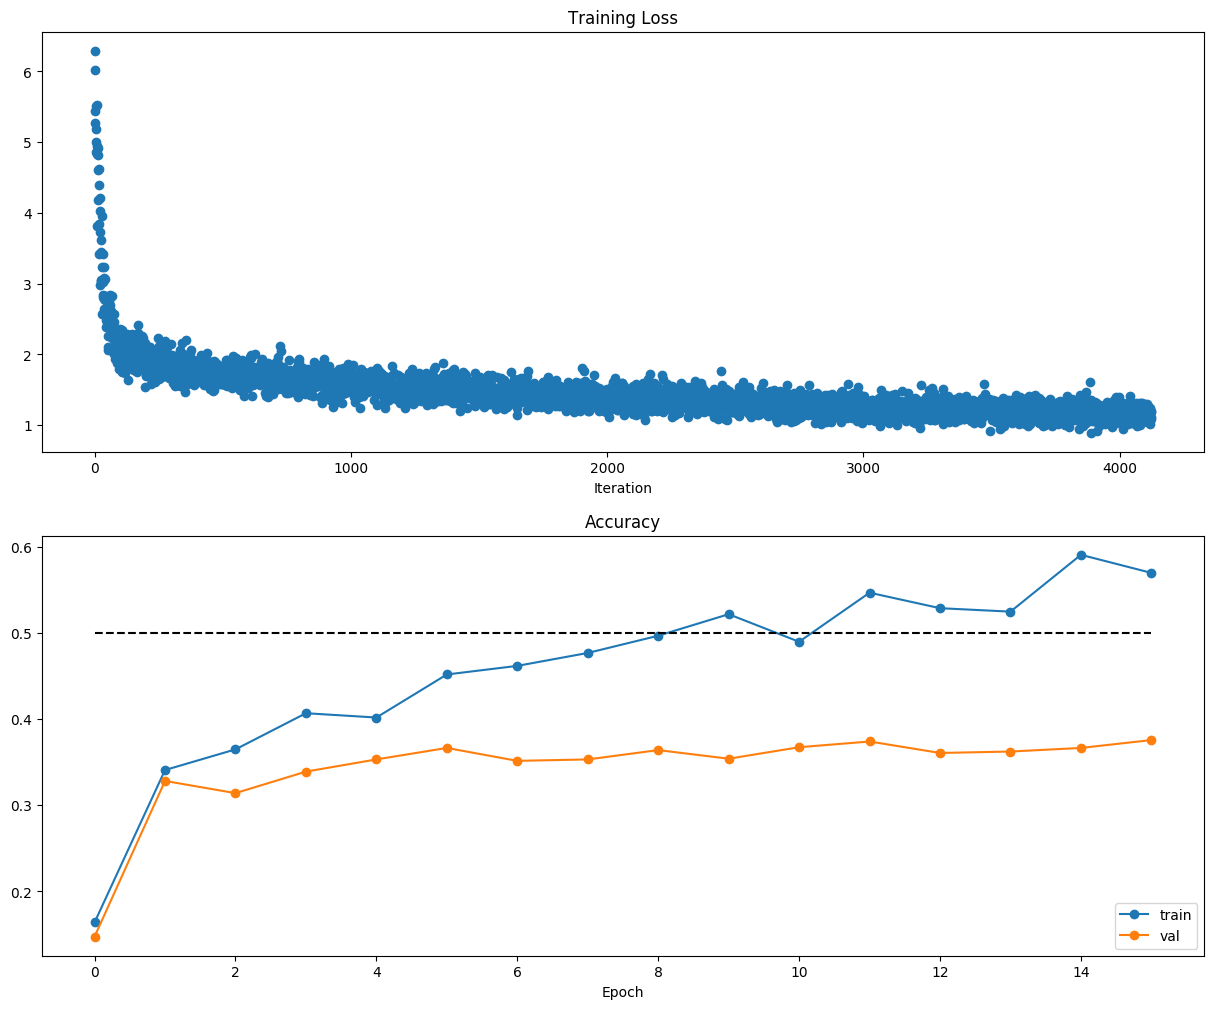
\includegraphics[scale = 0.32]{../nets/optimal_learning_rate/diagrams.png}}}  
  \end{figure}
  
\newpage  
\item \textbf{Using dropout}\\
  Now, keeping our optimal learning rate of 6.5e-5,
  we ran another grid search for dropout in the range (0.0, 1.0) to see if there was any improvement in the validation performance.
  Please find in the next section a plot of the validation accuracy rate at each dropout rate examined.
  As you can see, there is no improvement when using dropout, or perhaps the dropout rate is not independent with other hyperparameters
  such as the hidden layer's size or the momentum.
  Hence, it is possible that introducing a dropout rate requires us to recalibrate the learning rate.
  More on this in the last section!

\item \textbf{L2 vs dropout}:\\
  Let us now run a grid search to optimize L2 regularization,
  using the range (0.0, 1.0), to compare the performance against the dropout regularization.
  The highest validation accuracy rate obtained was 37.08\% with 0.85 L2 regularization constant.
  Please find below a plot of the validation accuracy rate at each L2 regularization rate tested, as well as for the dropout rate.
  It seems that the L2 rate is performing better than the dropout rate.
  In fact, as we increase the dropout rate from 0.0 to 1.0, we see an almost constant drop in performance.
  On the other hand, our model is doing better with an L2 regularization constant of 0.8 than without any.
  
  \begin{figure}[!ht]
    \centering
    \subfloat[Optimizing the dropout rate]{{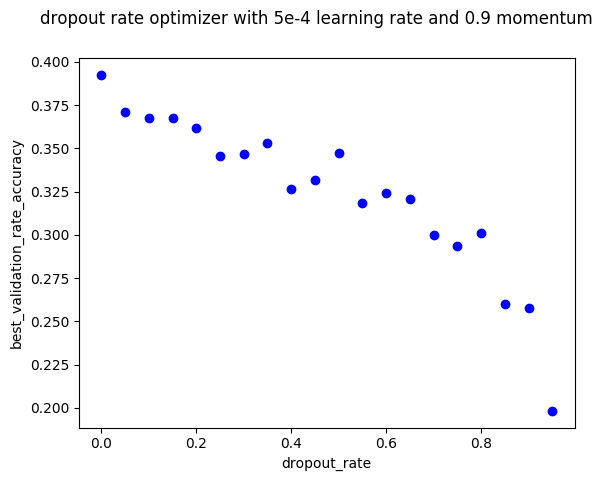
\includegraphics[scale = 0.40]{../src/optimizers/outputs/grid_search/dropout_rate.png}}}
    \qquad
    \subfloat[Optimizing the L2 rate]{{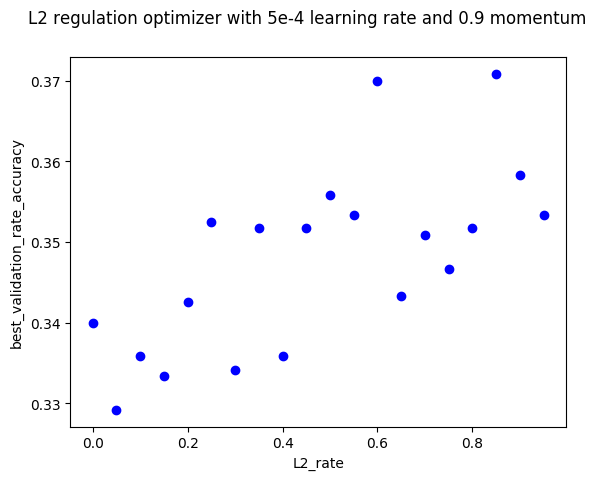
\includegraphics[scale = 0.40]{../src/optimizers/outputs/grid_search/L2_rate.png}}}
\end{figure}
  
\item \textbf{Optimizing the topology of the layer}:\\
  Thus far, we have assumed that a neural net's hyperparameters are independent variables.
  Yet our experiences thus far have shown us that this is a false assumption.
  To optimize the topology of the layer, we have instead decided to run a random search,
  letting every hyperparameter be randomly drawn (within its respective range as defined in previous sections).
  This removes the previous false assumption of hyperparameter variable independence.
  Given random search's potential for parallel computing, we used Imperial's \emph{condor} setup to send our random search program
  to all computers in the lab, training over 20,000 nets.
  We have found the optimal set of parameters to be:\\
  Please find below plots of accuracy and loss generated
  while training a network on this optimal set of parameters.

  
\item \textbf{Performance metrics of network trained with the optimal set of parameters}:\\
  Having trained a network on the optimal set of parameters in the previous section,
  we begin by presenting our model's classification error rates on each set.
  \include*{../nets/optimal_net/info}
  we now set out to test this model on the FER2013's testing set.
  Please find below a confusion matrix, precision and recall rates, as well as F1 scores per class.
  \begin{figure}[h]
  \begin{center}
    \caption{Confusion Matrix for test dataset}
    \begin{tabular}{ | l || c | c | c | c | c | c | c |}
    \hline
          & Angry 1 & Disgust 2 & Fear 3 & Happy 4 & Sad 5 & Surprise 6 & Neutral 7 \\ \hline \hline
        Angry 1 & 162 & 2 & 47 & 77 & 66 & 18 & 95 \\ \hline
        Disgust 2 & 11 & 14 & 5 & 10 & 8 & 1 & 7 \\ \hline
        Fear 3 & 67 & 2 & 141 & 74 & 79 & 41 & 92 \\ \hline
        Happy 4 & 76 & 1 & 56 & 543 & 81 & 33 & 105 \\ \hline
        Sad 5 & 104 & 7 & 81 & 108 & 198 & 20 & 135 \\ \hline
        Surprise 6 & 27 & 2 & 55 & 39 & 22 & 231 & 39 \\ \hline
        Neutral 7 & 76 & 6 & 53 & 102 & 92 & 32 & 246 \\ \hline
    \end{tabular}
    \label{fig:confusionMatrix}
\end{center}
\end{figure}


\begin{figure}[h]
\begin{center}
\caption{Recall and Precision Rates for test dataset}
\begin{tabular}{ | l || c | c | c | c | c | c | c | }
  \hline
                       & Angry 1 & Disgust 2 & Fear 3 & Happy 4 & Sad 5 & Surprise 6 & Neutral 7 \\ \hline \hline
        Avg Recall(\%) & 34.690 725.000 728.427 760.670 730.322 755.663 740.527 \\ \hline
        Avg Precision(\%) & 30.975 741.176 732.192 756.978 736.264 761.436 734.214 \\ \hline
        F\textsubscript{1} Measure(\%) & 32.727 731.111 730.193 758.766 733.028 758.407 737.104 \\ \hline
    \end{tabular}
    \label{fig:averageRecall}
\end{center}
\end{figure}




  

  
  
  
  
\item \textbf{How to retrieve our best trained model}:\\
  You may retrieve and test our best trained model using our test.py file.
  Thank you.
\end{itemize}
  
